\section{Results}
\label{sec:results}

\subsection{Sensitivity}
 show impact of HM DY on PDFs using sensitivity studies based on
pseudo-data, for which we only use the data uncertainties, while central 
value are fixed:
 HERA I+II vs HERA I+II + HMDY --> see the sensitivity plots from the previous email


conclusion: HMDY data has a large impact on photonPDF 



\subsection{PDF Fits}

In order to make a full PDF fit the  ATLAS Drell-Yan data data are fitted together with the final combined inclusive 
cross section data from HERA~\cite{hera}. The HERA data provide information on the quark/antiquark and gluon content of 
the proton and the Drell-Yan data add information on the photon content of the proton. 
The NLO and NNLO pQCD predictions are fitted to the data using the xFitter open source pQCD fitting platform~\cite{xFitter}.
The DGLAP equations~\cite{dglap} are solved using the programme QCDNUM which has been modified to include 
the photon PDF in the proton~\cite{qcdnum}.
The DGLAP equations yield the PDFs at all scales if they are input as finctions of $x$ at a starting scale $Q^2_0$, which 
should be large enough that perturbative QCD can be assumed to be valid. For the present analysis this value is chosen
to be $Q^2_0 = 7.5~$GeV$^2$. This is also the value chosen for the minimum value of $Q^2$ for data entering the fit.
The charm and beauty masses are chosen to be $m_c=1.47~$GeV and $m_b=4.5~$GeV following the HERA analysis. 
The value of $\alpha_s(M_Z)$ is chosen to be $\alpha_s(M_Z)=0.118$~\cite{PDG}. 
The value of $Q^2_0$ is above the charm mass squared, however a version of the programme 
is used which displaces the charm threshold from the charm mass~\cite{charmthresh} such that the threshold is at $Q^2_0$.
The form of the $\chi^2$ used for the fit is that defined in the H1 paper~\cite{h1chisqdef}. 
Alternative forms have also been tried with no significant difference to our results.
 
The PDF parametrisation input at $Q^2_0$ is determined by the technique of saturation of the $\chi^{2}$~\cite{h1chisqsat}.
The parametrised PDFs are the valence distributions $xu_{v}$ and $xd_{v}$, the gluon distribution $xg$, and the \textit{u}-type and \textit{d}-type sea, $x\bar{U}$, $x\bar{D}$, where $x\bar{U} = x\bar{u}$ and $x\bar{D} = x\bar{d} + x\bar{s}$, and finally the photon distribution $x\gamma$. The following standard functional form is used to parametrise them:
\begin{equation}
xf(x) = Ax^{B}(1-x)^{C}(1+Dx+Ex^{2})
\end{equation}
where the normalisation parameters $A_{u_{v}}$, $A_{d_{v}}$ and $A_{g}$ are constrained by the number sum-rules and the 
momentum sum-rule, respectively. The \textit{B} parameters $B_{\bar{U}}$ and $B_{\bar{D}}$ are set equal, such that there 
is a single \textit{B} parameter for the sea distribution. The data are not sensitive to the 
strangeness content of the proton which is thus set such that $x\bar{s} = 0.5\bar{D}$, following the ATLAS 
analysis~\cite{atlasstrange}. The further constraint $A_{\bar{U}} = 0.5 A_{\bar{D}}$ is imposed such that $\bar{u}=x\bar{d}$ as $x \to 0$.
The \textit{D} and \textit{E} parameters are introduced one by one until no significant 
improvement in $\chi^{2}$ is found. 

 For the NNLO fit a $\chi^{2}/ndf = 1.18$, with a partial $\chi^2/ndp = 1.15$ for the high-mass Drell-yan data [{\it update with final numbers}], is achieved for the following parametrisation, which has 11 parameters for the quarks and gluons and 5 parameters for the photon:
\begin{eqnarray}
xu_v(x) = A_{u_v}x^{B_{u_v}}(1-x)^{C_{u_v}}(1+E_{u_v}x^{2}), \\
xd_v(x) = A_{d_v}x^{B_{d_v}}(1-x)^{C_{d_v}}, \\
x\bar{U}(x) = A_{\bar{U}}x^{B_{\bar{U}}}(1-x)^{C_{\bar{U}}}, \\
x\bar{D}(x) = A_{\bar{D}}x^{B_{\bar{D}}}(1-x)^{C_{\bar{D}}}, \\
xg(x) = A_{g}x^{B_{g}}(1-x)^{C_{g}}(1+E_{g}x^{2}), \\
x\gamma(x) = A_{\gamma}x^{B_{\gamma}}(1-x)^{C_{\gamma}}(1+D_{\gamma}x+E_{\gamma}x^{2}) \\
\end{eqnarray}
The parametrisation for HERA data differs from that of the HERAPDF2.0 PDF since the starting scale $Q^2_0$ is higher and the additional negative term in the gluon parametrisation is not necessary.
Parametrisation and model uncertainties are considered according to the HERAPDF 
procedure~\cite{hera} 
by adding extra terms which make little difference to the $\chi^2$ of the fit, but which can change the shape of the PDFs. Additonal parameters considered are: the extra negative term for the gluon; $D_{u_v}$, $D_{\bar{u}}$ and $E_{\bar{d}}$. Model variations considered are the variation of: 
$m_b$ from 4.25 to 4.75 GeV; $m_c$ from 1.41 to 1.53 GeV;  $Q_0^2$ up to 10 GeV$^2$; 
$Q_{cut}^2$ up to 10 GeV$^2$; the strangeness fraction down to $f_s=0.4$; the value of $\alpha_s(M_Z)$ from 0.116 to 0.120.

Fig.~\ref{PDF_7.5GeV}
 shows the PDF distributions $x_{u_v},xd_{d_v},x\bar{u}, x\bar{d}, xg$ at $Q^{2}$ = 7.5$^{2}$ GeV$^{2}$,
including model and parametrisation uncertainties, while  Fig.~\ref{PDF_10000GeV} 
shows them at $Q^{2}$ = 10$^{4}$ GeV$^{2}$. {\it Add model and parametrisation variations, Use NNLO MC central}.
\begin{figure}
\includegraphics[width=7cm]{plots/uv_7_5.pdf} 
\includegraphics[width=7cm]{plots/dv_7_5.pdf} 
\includegraphics[width=7cm]{plots/gluon_7_5.pdf} 
\includegraphics[width=7cm]{plots/ubar_7_5.pdf} 
\includegraphics[width=7cm]{plots/dbar_7_5.pdf} 
\caption{NNLO PDF distributions at $Q^{2}$ = 7.5$^{2}$ GeV$^{2}$: (a) $u$ - valence; (b) $d$ - valence; (c) gluon; (d) $\bar{u}$; (e) $\bar{d}$ }
\label{PDF_7.5GeV}
\end{figure}
\begin{figure}
\includegraphics[width=7cm]{plots/uv_10000.pdf} 
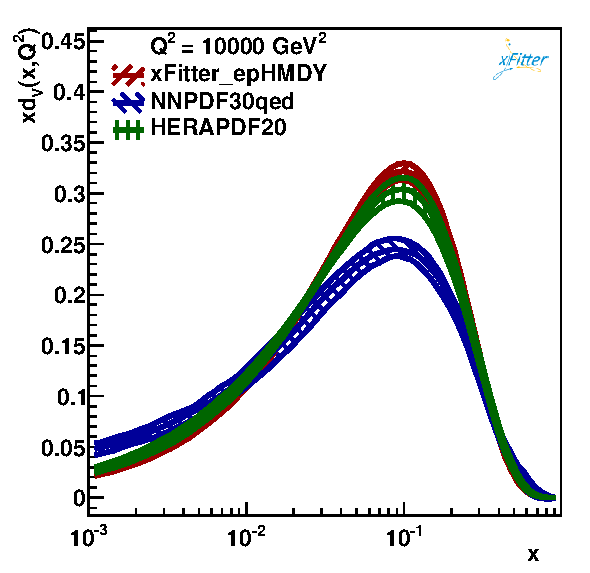
\includegraphics[width=7cm]{plots/dv_10000.pdf} 
\includegraphics[width=7cm]{plots/gluon_10000.pdf} 
\includegraphics[width=7cm]{plots/ubar_10000.pdf} 
\includegraphics[width=7cm]{plots/dbar_10000.pdf} 
\caption{NNLO PDF distributions at $Q^{2}$ = 10000$^{2}$ GeV$^{2}$: (a) $u$ - valence; (b) $d$ - valence; (c) gluon; (d) $\bar{u}$; (e) $\bar{d}$}
\label{PDF_10000GeV}
\end{figure}
In these figures comparisons are made to the NNPDF3.0PDF set and the HERAPDF2.0 set.
The shape of the $xd_{u_v}$ distribution is close to that of HERAPDF2.0 
because of the dominance of HERA data in the fit. 


Fig.~\ref{hmDY_2D} 
shows the comparison between the high-mass Drell-Yan double differential distribution and 
the predictions.
\begin{figure}
\centering
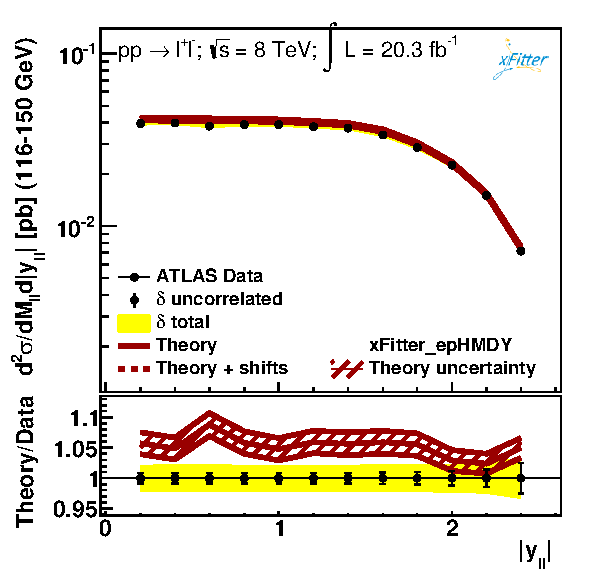
\includegraphics[width=7cm]{plots/data_1.pdf} 
\includegraphics[width=7cm]{plots/data_2.pdf} 
\includegraphics[width=7cm]{plots/data_3.pdf} 
\includegraphics[width=7cm]{plots/data_4.pdf} 
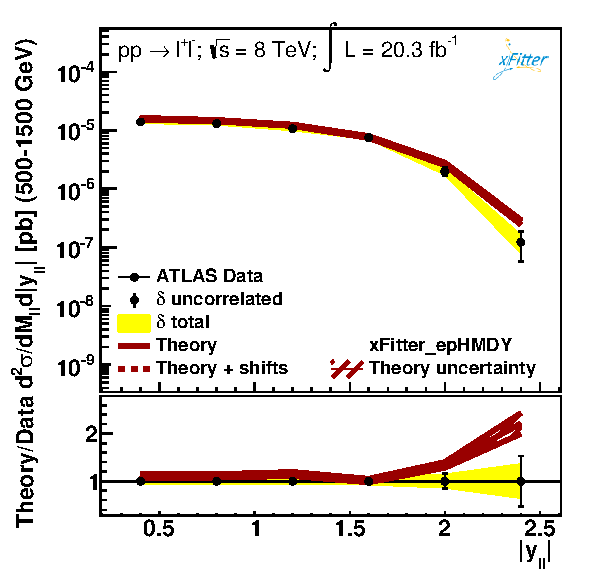
\includegraphics[width=7cm]{plots/data_5.pdf} 
\caption{Comparison between $\frac{d^{2}\sigma}{dm_{ll}d|y_{ll}|}$ for the high-mass Drell Yan data and the NNLo fit predictions.}
\label{hmDY_2D}
\end{figure}
The $\chi^{2}$ values for the high-mass Drell Yan data and the output parameters from NNLO fit can be found in Table.~\ref{chi2_scan} 
and Table.~\ref{par_scan} 
respectively. 
\begin{figure}
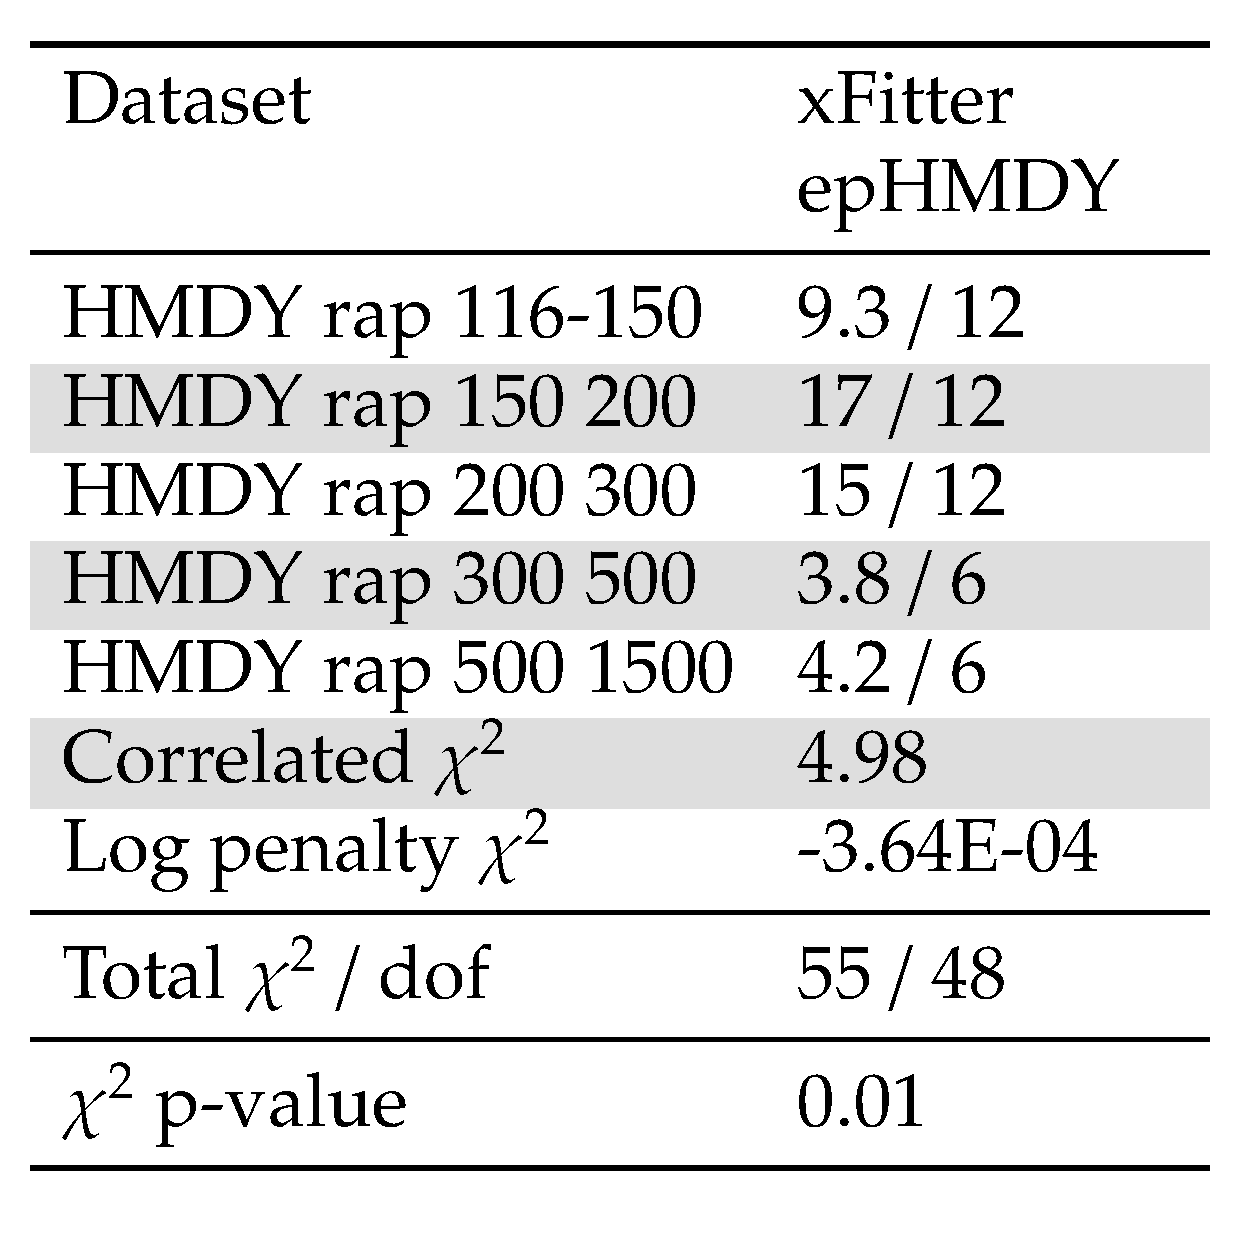
\includegraphics[width=14cm]{plots/chi2_hmDY.pdf} 
\caption{$\chi^{2}$ for high-mass Drell Yan data, for the NNLO fit}
\label{chi2_scan}
\end{figure}
\begin{figure}
\includegraphics[width=14cm]{plots/parameters.pdf} 
\caption{PDF parameters for the NNLO fit.}
\label{par_scan}
\end{figure}

The NNLO photon PDF distribution is shown 
both at the starting scale (7.5 GeV$^{2}$) and at 10$^{4}$ GeV$^{2}$ 
 in Fig.~\ref{photon}, where it is also compared to an NLO extraction of the photon distribution.
The $x$-range of the figure is restricted to the range of sensitivity of the high-mass drell-Yan data;
$0.045 < x < 0.35$. The NLO and NNLO photon PDFs are compatible over this range.
\begin{figure}
\includegraphics[width=7cm]{plots/photon_7_5.pdf} 
\includegraphics[width=7cm]{plots/photon_10000.pdf} 
\caption{Comparison between the photon PDF distributions at NNLO and NLO: (a) at the starting scale; (b) at the evolved scale.}
\label{photon}
\end{figure}

Fig.~\ref{photon_zoom} 
shows the photon distribution in the restricted range compared to the NNPDF3.0qed NNLO photon PDF.
The uncertainties are considerably reduced. The comparison is shown at scale 100 GeV$^{2}$ and 
at 10$^{4}$ GeV$^{2}$, where the value of 100 GeV$^{2}$ is chosen such that comparisons can also be 
made to the LUXqed~\cite{luxqed} photon PDF, which is only defined above this scale.  The 
HKR photon PDF~\cite{hkr} is also shown in this figure. The fit predictions from the present analysis
agree  with the LUXqed and the HKR photon PDFs at the 1-$\sigma$ level. 


\begin{figure}
\includegraphics[width=7cm]{plots/photon_comp_100.pdf} 
\includegraphics[width=7cm]{plots/photon_comp_10000.pdf} 
\caption{Comparison between the NNLO photon PDF distributions for the present analysis, NNPDF3.0QED, LUXqed, HKR: (a) at scale 100 GeV$^{2}$; (b) at the evolved scale 10000 GeV$^{2}$.}
\label{photon_zoom}
\end{figure}

